\ExTitle{5}
\begin{aufgabe}
\end{aufgabe}

\begin{enumerate}[a)]
	\item Warum verwendet man die PCA?\\
	Die Aufgabe von PCA besteht darin, Merkmale zusammenzufassen und somit Dimensionen meiner Daten zu reduzieren. Das bringt zwar in jedem Fall einen Fehler mit sich, allerdings ist der PCA so konzipiert, dass der entstehende Fehler bei minimiert wird. Das ist dann nützlich, wenn ich \\
	(\textbf{1}) zu viele Dimensionen für relativ wenig Daten habe. Dann ist das einfach undurchschaubar. Somit hilft die PCA, indem die Streumatrix den Rang und somit auch $\min\{n,p\}$ Eigenwerte (Komponenten) besitzt, wobei $n$ die Anzahl der Daten und $p$ die Anzahl der Merkmale sind. Ein weiterer Grund: \\
	(\textbf{2}) Wenn einige Merkmale eine gewisse Redundanz besitzen, das heißt, dass sie stark korrelierend sind. Dann lassen sie sich zusammenfassen und die PCA arbeitet dabei schnell, einfach und effizient, sodass wir eine gute \underline{Repräsentation} der Daten bekommen im Sinne der Varianz.
	\item \underline{Ziel von PCA:} Der Algorithmus möchte die Daten auf die größte Varianz reduzieren. Dazu berechnet er die Eigenwerte und -vektoren der Streumatrix \underline{aller} Daten und schaut, welche groß - also relevant - sind. Die entscheiden dann die einzelnen Komponenten in absteigender Reihenfolge und maximieren somit die Varianz der Daten. Insofern liegt da der große Unterschied zu \underline{LDA}\\
	LDA berechnet sowohl die Mittelwerte, als auch die within-class und between-class Streumatrizen. Die Eigenwerte von $A_{within}^{-1}\cdot A_{between}$ geben nun die Diskriminanten für den neuen Unterraum an und dann schiebt LDA alles rüber. Maximiert wird hiermit die Streuung zwischen den Klassen, wobei die Streuung innerhalb einer Klasse minimiert wird ($J(w)$ im Skript). Es reicht nicht, sie einzeln zu maximieren, da ansonsten schlicht und einfach nichts neues passiert. Somit ergibt sich im neuen Schaubild eine Klassifizierungsmöglichkeit. 
 	\item Die \underline{within-class} Streumatrix ist die Summe der einzelnen Streumatrizen pro Klasse ($\sum (x-m)(x-m)^t$) und beschreibt, wie stark die Daten innerhalb einer Klasse variieren.
 	\item Die \underline{between-class} Streumatrix beschreibt, wie weit die einzelnen Klassenmittelwerte vom globalen Mittelwert abweichen und gibt somit an, wie die Klassen beieinander liegen.
	\item PCA gilt hierbei als ein \textit{unsupervised} Verfahren, da es sich ausschließlich für die Varianzmaximierung interessiert. Im Gegensatz dazu berechnet LDA die Richtungen (Lineare Diskriminanten), um die Daten möglichst weit in Klassen aufzuteilen. Somit gilt LDA als ein \textit{supervised} Verfahren.
\end{enumerate}

\begin{aufgabe}
\end{aufgabe}

Einzuzeichnen sind in die Grafiken die erste Komponente nach PCA, also die Richtung, in der erst mal am stärksten gestreut wird. Das macht dann nämlich den ersten Eigenvektor laut dem PCA Algoritmus aus. In Rot wurde der erste Komponentenvektor eingetragen.

\begin{center}
	\fbox{
		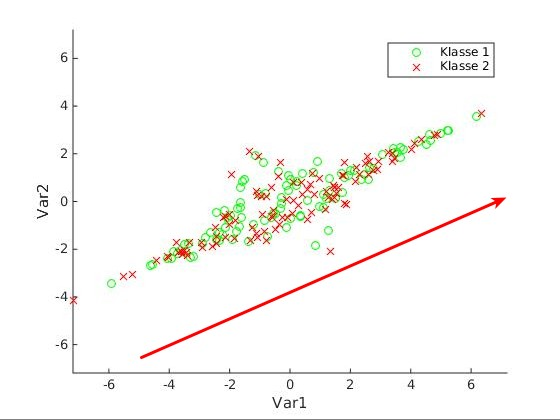
\includegraphics[width=0.4\textwidth]{05/data/img1}
	}\\
\end{center}
Hier sind die Daten verstreut in einer Punktemenge, wobei schlecht unterschieden werden kann. Der PCA bietet sich an, durch einen PCA würde die Streuung verdeutlicht werden und das wäre mit einer fortsetzenden LDA förderlich für die Klassifizierung.
\begin{center}
	\fbox{
		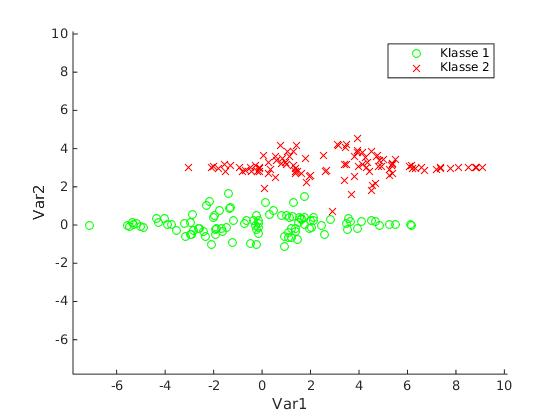
\includegraphics[width=0.7\textwidth]{05/data/img2}
	}\\
\end{center}
Hier würde ein PCA die bereits getrennten Klassen wieder zusammenschmeißen, was wiederum nicht förderlich für eine Klassifizierung wäre. Auch wäre ein PCA hier nicht angebracht, da die Daten so separiert sind, wie sie sind.
\begin{center}
	\fbox{
		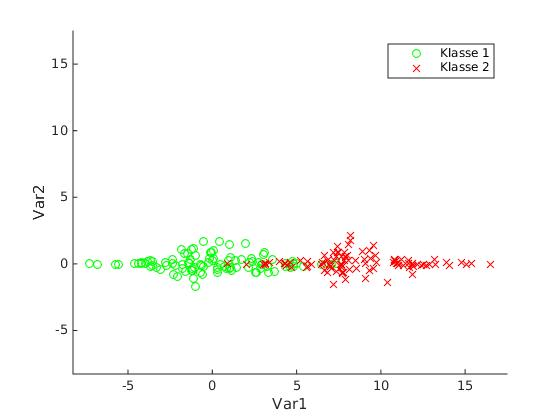
\includegraphics[width=0.7\textwidth]{05/data/img3}
	}\\
\end{center}
Hier wäre ein PCA angebracht, um die "Grenzen der Klassen" ein wenig besser zu durchforsten. Es könnte insofern förderlich für die Klassifizierung sein, dass wir dann anschließend durch LDA weniger Fehler begehen.
\begin{center}
	\fbox{
		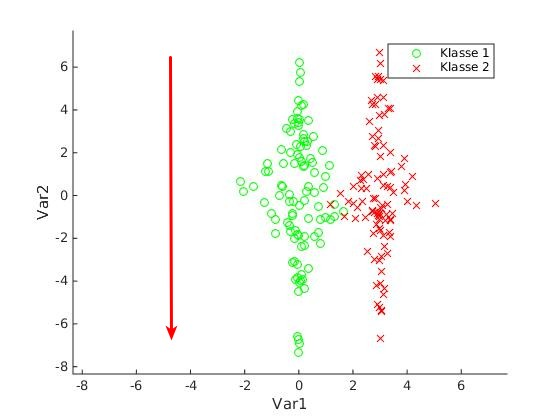
\includegraphics[width=0.7\textwidth]{05/data/img4}
	}\\
\end{center}
